\documentclass[11pt]{beamer}
\usetheme{Boadilla}
\usepackage[utf8]{inputenc}
\usepackage[french]{babel}
\usepackage[T1]{fontenc}
\usepackage{amsmath}
\usepackage{amsfonts}
\usepackage{amssymb}
\usepackage{graphicx}
\usepackage{hyperref}
\author[GOFFART M. \and JORIS O.]{GOFFART Maxime \and JORIS Olivier}
\title{Codage de Prüfer}
%\setbeamercovered{transparent} 
%\setbeamertemplate{navigation symbols}{} 
%\logo{} 
%\institute{} 
\date{2019 - 2020} 
%\subject{} 
\begin{document}

\begin{frame}
\titlepage
\end{frame}

\begin{frame}
Table des matières :
\tableofcontents
\end{frame}

\section{Origine du codage de Prüfer}

\begin{frame}{Origine du codage de Prüfer}

\begin{tabular}{cl}  
         \begin{tabular}{c}
         		  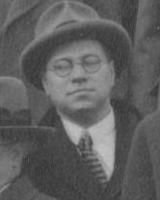
\includegraphics[height=4cm, width=3cm]{heinzPrufer.jpg}
           \end{tabular}
           & \begin{tabular}{l}
             \parbox{0.6\linewidth}{
             Les suites du Prüfer ont été inventées par Heinz Prüfer en 1918.\\\\
			Heinz Prüfer était un mathématicien allemand spécialisé en algèbre et en théorie des groupes.
   			}
         \end{tabular}  \\
\end{tabular}

\tiny{\url{https://en.wikipedia.org/wiki/Heinz_Prüfer}}
\end{frame}

\begin{frame}{Origine du codage de Prüfer}

Les codages de Prüfer permettent de représenter de manière condensée un arbre.\\
\vspace{1cm}
Un exemple sera donné plus loin.
\end{frame}


\section{Utilité des codages de Prüfer}

\subsection{1\iere{} utilité}
\begin{frame}
\tableofcontents[currentsection, currentsubsection]
\end{frame}

\begin{frame}
\frametitle{Utilité des codages de Prüfer}

\begin{center}
\LARGE{Utilité dite mathématique}
\end{center}

\end{frame}

\begin{frame}
\frametitle{Utilité des codages de Prüfer}
\framesubtitle{Mathématique}

La raison pour laquelle ils ont été inventés :\\
\vspace{0.3cm}
\begin{center}
\textbf{Démontrer la formule de Cayley}
\end{center}
\pause
\vspace{0.2cm}
\begin{block}{Formule de Cayley}
Soit n $>$ 1. On peut construire n$^{\text{n}-2}$ arbres différents constitués de n sommets numérotés.
\end{block}

\end{frame}

\subsection{2\ieme{} utilité}
\begin{frame}
\tableofcontents[currentsection, currentsubsection]
\end{frame}

\begin{frame}
\frametitle{Utilité des codages de Prüfer}

\begin{center}
\LARGE{Utilité dite informatique}
\end{center}

\end{frame}

\begin{frame}
\frametitle{Utilité des codages de Prüfer}
\framesubtitle{Informatique}

\begin{center}
\textbf{Stocker un arbre en minimisant la mémoire utilisée}
\end{center}
\end{frame}

\begin{frame}
\frametitle{Utilité des codages de Prüfer}
\framesubtitle{Informatique}

Il y a 3 manières de représenter un arbre dans la mémoire d'un ordinateur :\\

\begin{enumerate}
\item[$\bullet$]Par sa matrice d'adjacence
\item[$\bullet$]Par listes d'adjacences
\item[$\bullet$]Par codage de Prüfer
\end{enumerate}
\end{frame}

\begin{frame}
\frametitle{Utilité des codages de Prüfer}
\framesubtitle{Informatique}

Soit l'arbre suivant :\\
\begin{figure}[!ht] \center
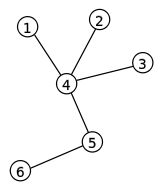
\includegraphics[scale=0.40]{exempleArbre.png}
\end{figure}
\begin{center}
\tiny{\url{https://fr.wikipedia.org/wiki/Codage_de_Prüfer}}
\end{center}

Notons cet arbre A = ($\#$V, $\#$E).
Nous allons représenter cet arbre des 3 manières différentes.
\end{frame}

\begin{frame}
\frametitle{Utilité des codages de Prüfer}
\framesubtitle{Informatique}

\begin{table}[]
\centering
\begin{tabular}{l|l|l}
Matrice d'adjacence   & Listes d'adjacences   & Suite de Prüfer      \\
\multicolumn{1}{c|}{$\begin{array}{cccccc}
x & x & x & 1 & x & x \\ 
x & x & x & 1 & x & x \\ 
x & x & x & 1 & x & x \\ 
1 & 1 & 1 & x & 1 & x \\ 
x & x & x & 1 & x & 1 \\ 
x & x & x & x & 1 & x
\end{array}$ } & \multicolumn{1}{c|}{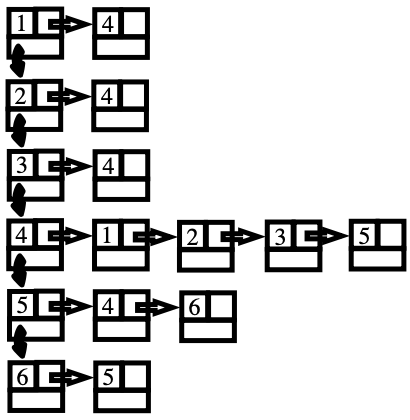
\includegraphics[scale=0.30]{listesAdj.png}} & \multicolumn{1}{c}{4 4 4 5}
\end{tabular}
\end{table}
\end{frame}

\begin{frame}
\frametitle{Utilité des codages de Prüfer}
\framesubtitle{Informatique}

Quelle quantité de mémoire est nécessaire pour stocker cet arbre ?
\vspace{0.3cm}
\begin{enumerate}
\item[$\bullet$]Par sa matrice d'adjacence : $(\# V)^2$
\item[$\bullet$]Par listes d'adjacences : $\# V + \# E$
\item[$\bullet$]Par codage de Prüfer : $\# V - 2$
\end{enumerate}
\vspace{1cm}
Pour les grands arbres, le codage de Prüfer est très intéressant.
\end{frame}

\section{Exemples}

\subsection{Codage}
\begin{frame}
\tableofcontents[currentsection, currentsubsection]
\end{frame}

\begin{frame}
\frametitle{Exemples}
\framesubtitle{Codage}

\begin{center}
Voir \textit{Jupyter Notebook}\\
\vspace{3cm}
\tiny{\url{http://localhost:8888/notebooks/Codage\%20Prufer\%20exemple.ipynb\#}}
\end{center}
\end{frame}

\subsection{Décodage}
\begin{frame}
\tableofcontents[currentsection, currentsubsection]
\end{frame}

\begin{frame}
\frametitle{Exemples}
\framesubtitle{Décodage}

\begin{center}
Voir \textit{Jupyter Notebook}\\
\vspace{3cm}
\tiny{\url{http://localhost:8888/notebooks/Decodage\%20Prufer\%20exemple.ipynb}}
\end{center}
\end{frame}


\end{document}